\documentclass[10pt, oneside]{article}   	% use "amsart" instead of "article" for AMSLaTeX format

\usepackage{geometry}                		% See geometry.pdf to learn the layout options. There are lots.
\geometry{letterpaper}                   		% ... or a4paper or a5paper or ... 
%\geometry{landscape}                		% Activate for for rotated page geometry
%\usepackage[parfill]{parskip}    		% Activate to begin paragraphs with an empty line rather than an indent
\usepackage{graphicx}				% Use pdf, png, jpg, or eps§ with pdflatex; use eps in DVI mode
								% TeX will automatically convert eps --> pdf in pdflatex		
\usepackage{amssymb}
\usepackage{amsmath} %GF
\usepackage{siunitx} %VZ
%\usepackage{bbold} %VZ

\usepackage{framed} % GF serve a mettere la caption a roba che non è table o image
\usepackage{listings}
\usepackage{textcomp}
\lstset{
    tabsize=4,    
%   rulecolor=,
    language=C++,
        basicstyle=\scriptsize,
        upquote=true,
        aboveskip={1.5\baselineskip},
        columns=fixed,
        showstringspaces=false,
        extendedchars=false,
        breaklines=true,
        prebreak = \raisebox{0ex}[0ex][0ex]{\ensuremath{\hookleftarrow}},
        frame=single,
        numbers=left,
        showtabs=false,
        showspaces=false,
        showstringspaces=false,
        identifierstyle=\ttfamily,
        keywordstyle=\color[rgb]{0,0,1},
        commentstyle=\color[rgb]{0.026,0.112,0.095},
        stringstyle=\color[rgb]{0.627,0.126,0.941},
        numberstyle=\color[rgb]{0.205, 0.142, 0.73},
%        \lstdefinestyle{C++}{language=C++,style=numbers}’.
}

\title{GSSI - statistical and software tools for data analysis (M. Agostini)}
\author{Guido Fantini}
\date{}							% Activate to display a given date or no date

\usepackage{color}

\newcommand{\vz}[1]{{\sf\leavevmode\color{magenta}#1}}
\newcommand{\fv}[1]{{\bf\leavevmode\color{cyan}#1}}
\newcommand{\gf}[1]{{\sc\leavevmode\color{blue}#1}}


\begin{document}
\maketitle
%\section{}
%\subsection{}


\newpage
\tableofcontents %\newpage

\newpage %

\section{Coverage}

Let us consider a toy analysis where the distribution of the observable quantity $x$ in both the signal and the background hypothesis is known.
The observable is defined in the range $(-10,10)$ and its probability density function in the two cases is
$$ f_s(x) = \frac{1}{\sqrt{2\pi} \sigma} e^{-\frac{(x-\mu)^2}{2\sigma^2}} \quad \mathrm{where} \quad \mu = 0 \:\: \sigma = 1 $$
$$ f_b(x) = \frac{1}{20} $$

A frequentist analysis is performed for different combinations of \textit{true} signal and background expected counts in order to extract a confidence interval for the signal at $90\% \mathrm{C.L.} $. A coverage test is performed in each expected background condition as a function of the expected signal count and an overcoverage is observed when the \textit{true} number of signal events is below the sensitivity defined by the background. 

\subsection{Procedure}
Let us define the \textit{true} expected number of signal (background) events as $S (B)$.
Two background conditions were simulated: $B = 1$ (low background) and $B = 100$ (high background).
For each of these conditions a set of \textit{true} $S$ values was defined and the following procedure was performed:
\begin{itemize}
\item two random numbers $N_s$ and $N_b$ were extracted according to Poisson distributions of parameter $S$ and $B$ respectively (i.e. $Poisson(N_s | S)$ and $Poisson(N_b | B)$ ). Being a random process, even when the expected number of signal and background events is known exactly, the actual number of signal and background realizations fluctuates;
\item $N_s$ events (i.e. realizations of the random variable $x$ in the signal hypothesis) were generated from the $f_s$ distribution and added to an histogram;
\item $N_b$ events were generated from the $f_b$ distribution and added to the same histogram;
\item the histogram was fit with the distribution $f(x|S,B) = S f_s + B f_b$ where $S$ and $B$ are parameters. A binned likelihood was built in order to account for the poissonian fluctuations of the bin contents $\mathcal{L}(S,B) \doteq \prod_{bins} Poisson(counts_{bin} | \int_{bin}f(x|S,B)dx)$ and maximized globally (as a function of both $S$ and $B$) in order to find the best fit number of signal and background events as maximum likelihood estimators $\hat{S}$ and $\hat{B}$;
\item assuming the Wilks theorem applies (i.e. in the large sample limit) and the null model (the one defined by $\hat{S}$ and $\hat{B}$) is true, the log-likelihood ratio test statistics 
$$ t = -2log\frac{ \mathcal{L}(S,\hat{\hat{B}})}{\mathcal{L}(\hat{S},\hat{B})} $$
where $\hat{\hat{B}}$ is the value of $B$ that maximizes the likelihood as a function of $B$ only, has a chi-square distribution with one degree of freedom. This means that, once a confidence level is set, we can define an interval as the union of the $S$ values for which the test statistics is below some threshold $t_{max}$ such that 
$$\int_{t_{max}}^{\infty} f_t(t) dt = 1 - \mathrm{C.L.}$$
When the test statistics is below threshold, the hypothesis test between the null hypothesis ($\hat{B}$ and $\hat{S}$) and the alternate hypothesis ($S$ and $\hat{\hat{B}}$) would accept the null hypothesis.
Since we assume the Wilks' approximation holds, the threshold equals the $1 - \mathrm{C.L.}$ quantile of the $f(\chi^2,\nu = 1)$ distribution

$$ t_{max} = 2.7 \quad C.L. = 90\% $$
A $90 \%$ confidence interval was extracted according to this approximation.
\item the above procedure from the poisson generation of the number of events from the \textit{true} value to the extraction of the confidence interval was repeated $N_{try} = 10^4$ times;
\item for each repetition a check was performed whether the \textit{true} value of the signal events was contained in the confidence interval. The ratio between the number of successes and the number of trials yield an estimate of the coverage of the interval obtained with this method;
\item an estimation of the uncertainty on the coverage estimation was performed. The coverage estimator 

$$ \hat{c} = \frac{n_{inside}}{N_{try}}$$
is given by the ratio of a binomial variable $n_{inside}$ and a constant. Hence

$$ \sigma(\hat{c}) = \frac{1}{N_{try}} \sigma(n_{inside}) = \frac{\sqrt{c(1-c)}}{\sqrt{N_{try}}}$$
\end{itemize}
\subsection{Results}

The results of the procedure described in the previous section are reported below in Fig. \ref{fig:cov_b1} and \ref{fig:cov_b100}. An overcoverage is observed when the number of \textit{true} signal events is below the sensitivity. A very rough order-of-magnitude-estimate of the sensitivity can be obtained computing the square root of the number of expected background events in the "signal region" defined as $\pm 1 \sigma$ of the signal distribution i.e. $\sqrt{B / 6}$. In the low background case the sensitivity is up to $S \sim \sqrt{1/6} \sim 0.4$ and the problem is not visible (see Fig. \ref{fig:cov_b1}). In the high background case instead the sensitivity is up to $S \sim \sqrt{100/6} \sim 4$ and this is the reason why for $S = 1$ and $S=0.1$ an overcoverage is observed (see Fig. \ref{fig:cov_b100}). 
%% gotta check if this is the case! 
%% poisson + poisson = poisson
%% s = 0 + b = svario --> poisson(svario) --> gauss(svario,sqrt(svario)) --> vale wilks --> WTF!!

\begin{figure}[h!]
    \centering
    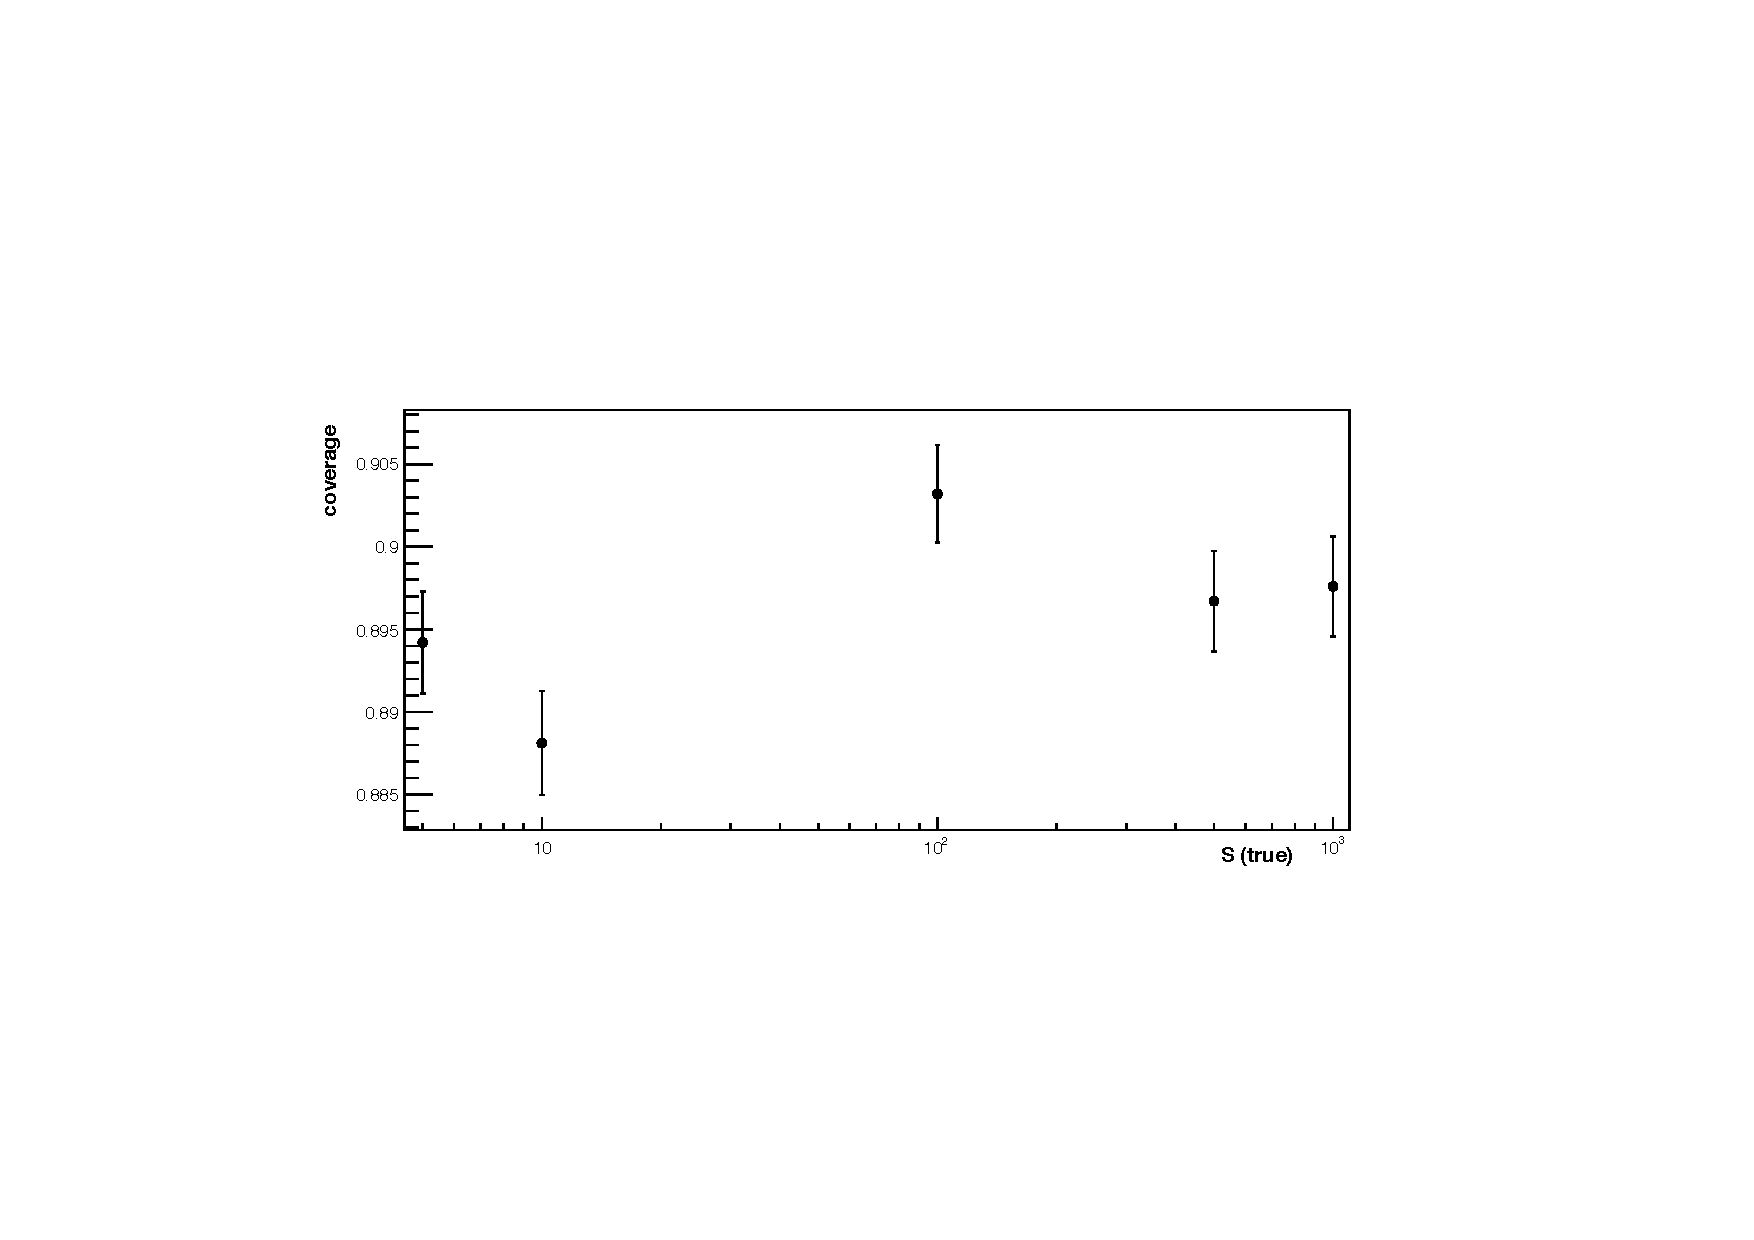
\includegraphics[width=\textwidth]{Ex1_b1.pdf}
    \caption{Coverage computation in the low background $(B = 1)$ case. $N_{try} = 10^4$ data samples generated.}
    \label{fig:cov_b1}
\end{figure}

\begin{figure}[h!]
    \centering
    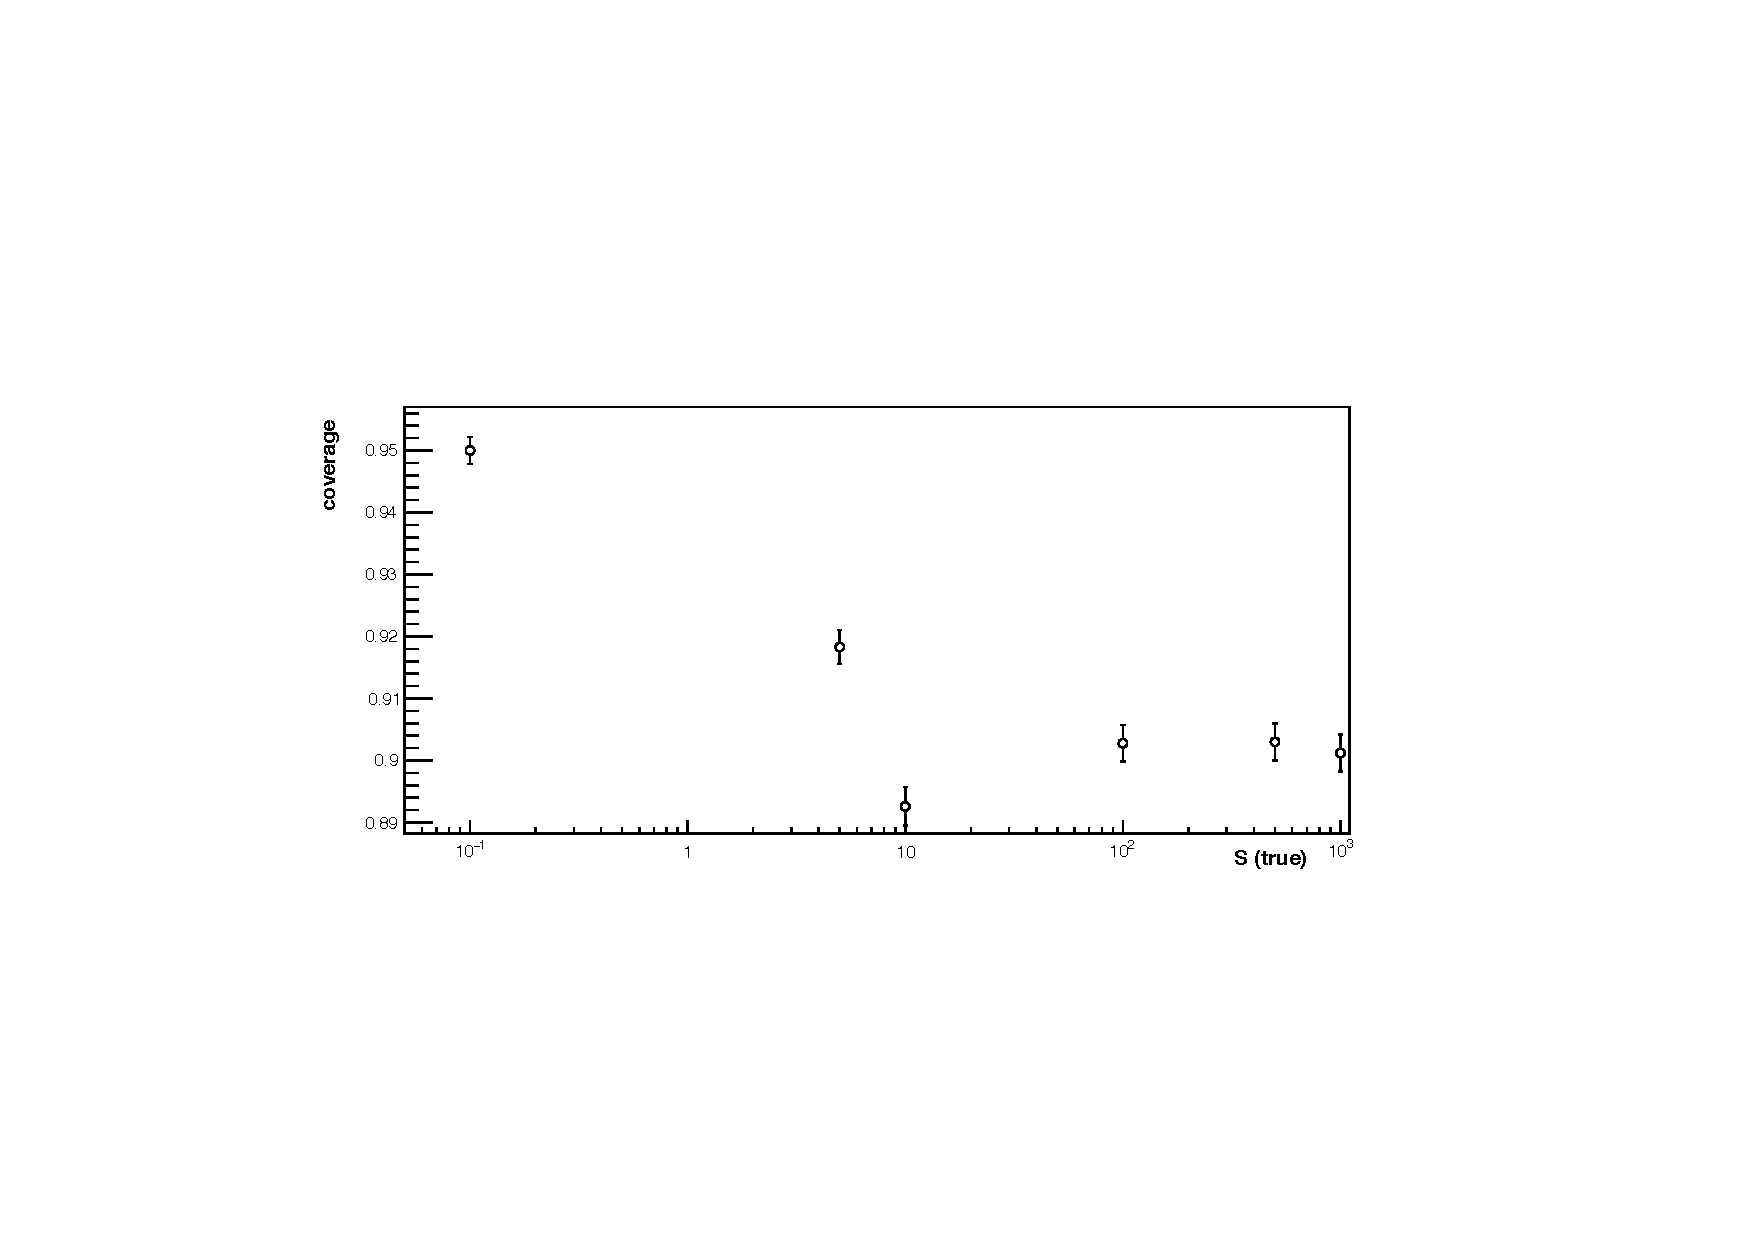
\includegraphics[width=\textwidth]{Ex1_b100.pdf}
    \caption{Coverage computation in the high background $(B = 100)$ case. $N_{try} = 10^4$ data samples generated.}
    \label{fig:cov_b100}
\end{figure}

\begin{figure}[h!]
    \centering
    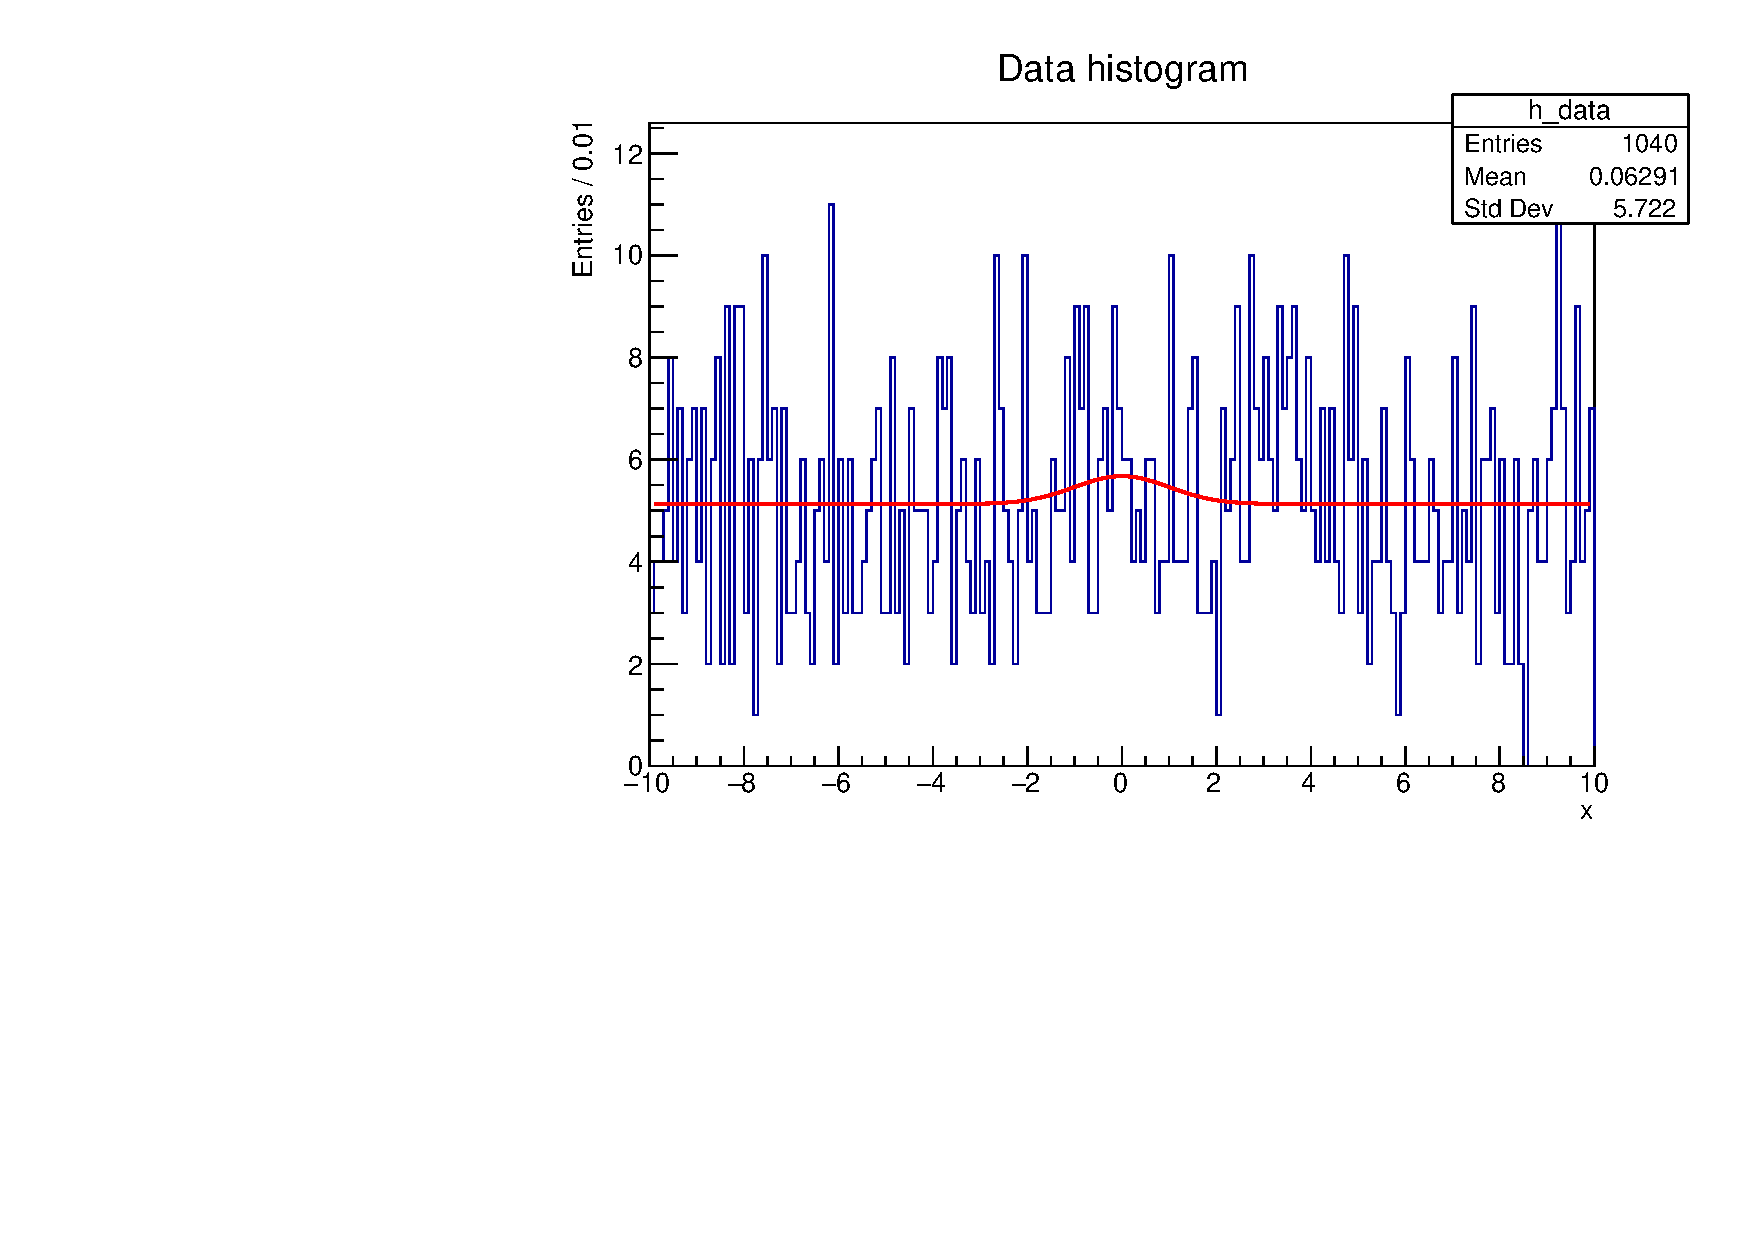
\includegraphics[width=\textwidth]{Events_S1B1000.pdf}
    \caption{Example of event generation (blue) and best fit function (red).}
    \label{fig:events_b1000}
\end{figure}

\begin{figure}[h!]
    \centering
    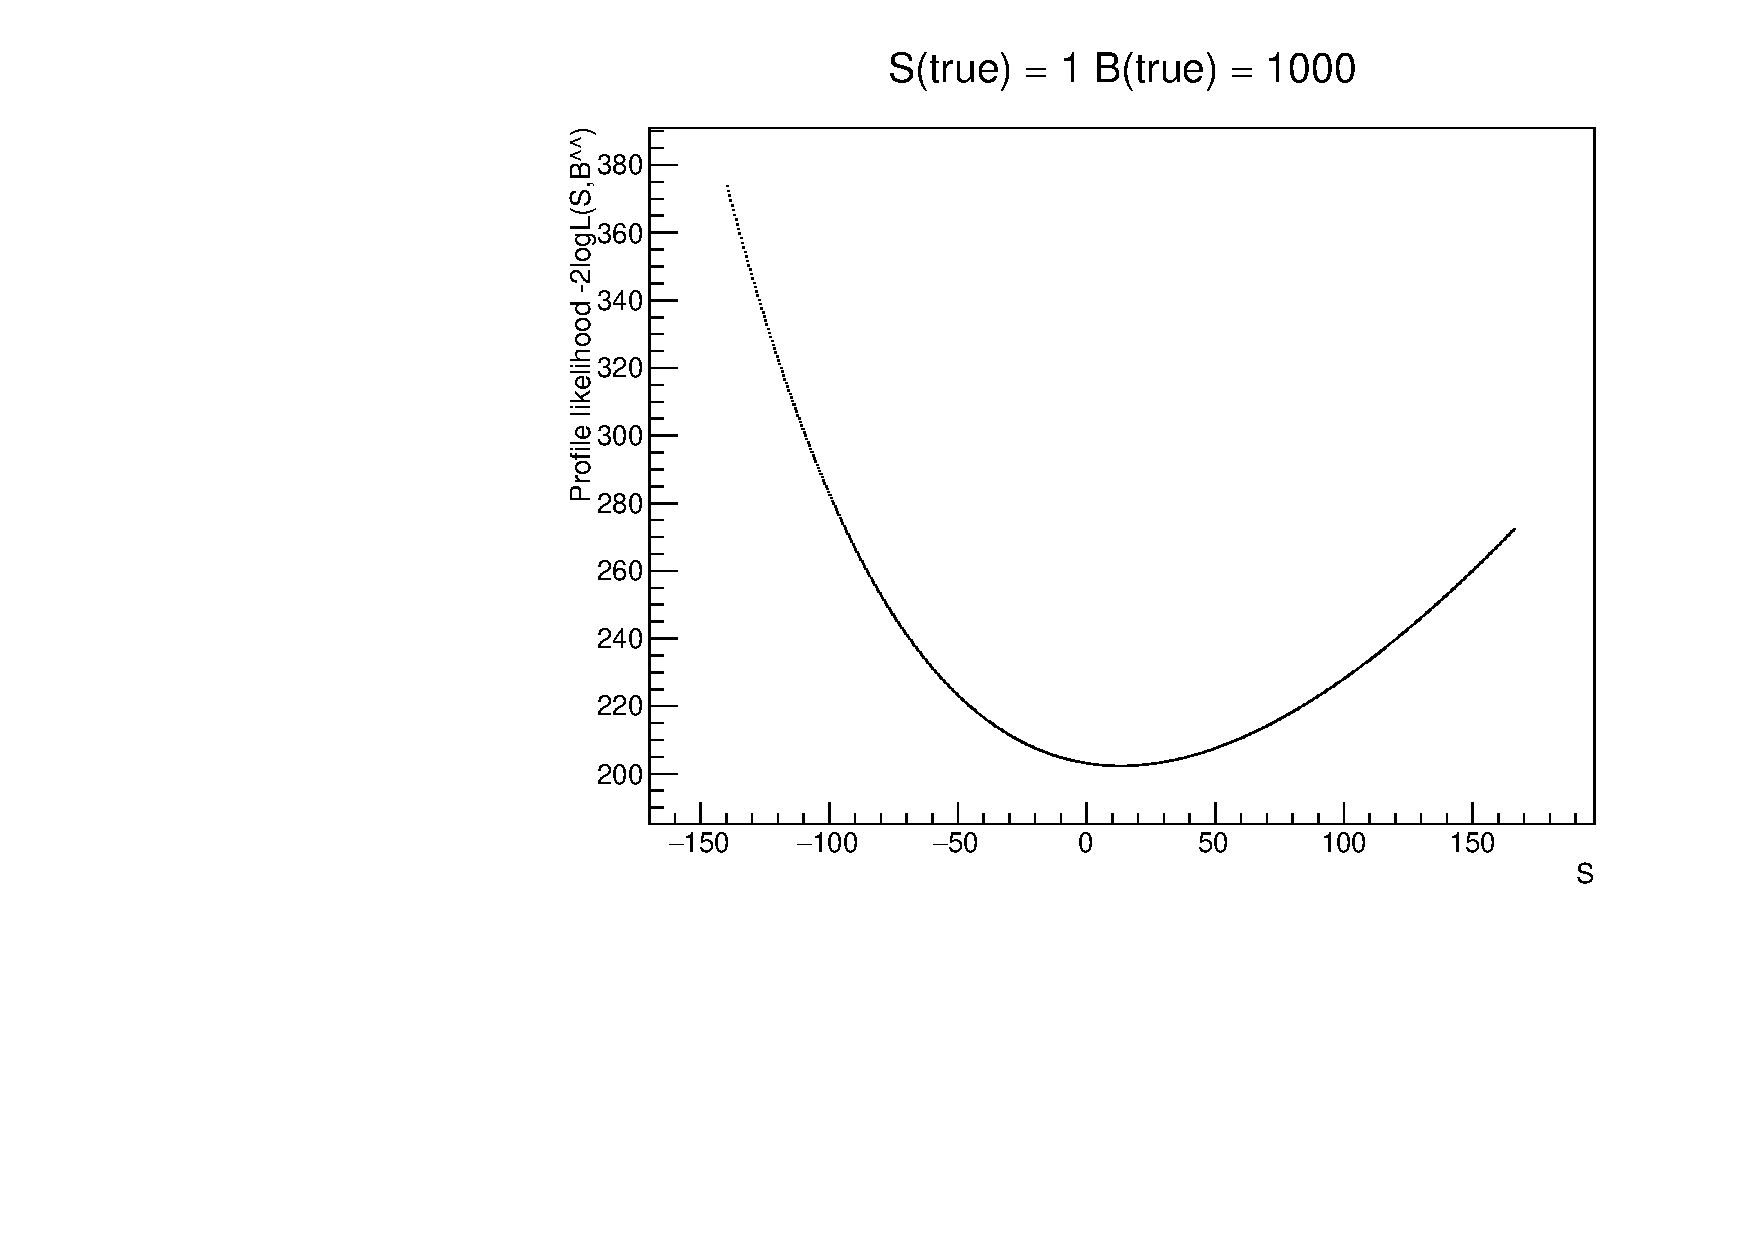
\includegraphics[width=\textwidth]{ProfileLikelihood_S1B1000.pdf}
    \caption{Example of profile likelihood $-2log(\mathcal{L}(S,\hat{\hat{B}}))$ as a function of the alternate signal $S$.}
    \label{fig:profileL_b1000}
\end{figure}

\newpage

\section{The distribution of the log-likelihood ratio}
In order not to assume the Wilks' approximation is valid or in all the situations in which actually it is not, the only way to compute the proper threshold for the test statistics and, as a consequence, to build the correct frequentist interval at a given $CL$ is to evaluate numerically the distribution of the test statistics and compute from that the desired quantile.
This is what was done for a sample of $N_{toy} = 10^5$ toy-MC datasets for true values of $B = 1000$ and $S = 100, 1000$ and $N_{toy} =10^6$ for the same background level and $S = 1, 10$. The quantile obtained in this way is reported in Fig. \ref{fig:threshold_b1000}.
\begin{figure}[h]
    \centering
    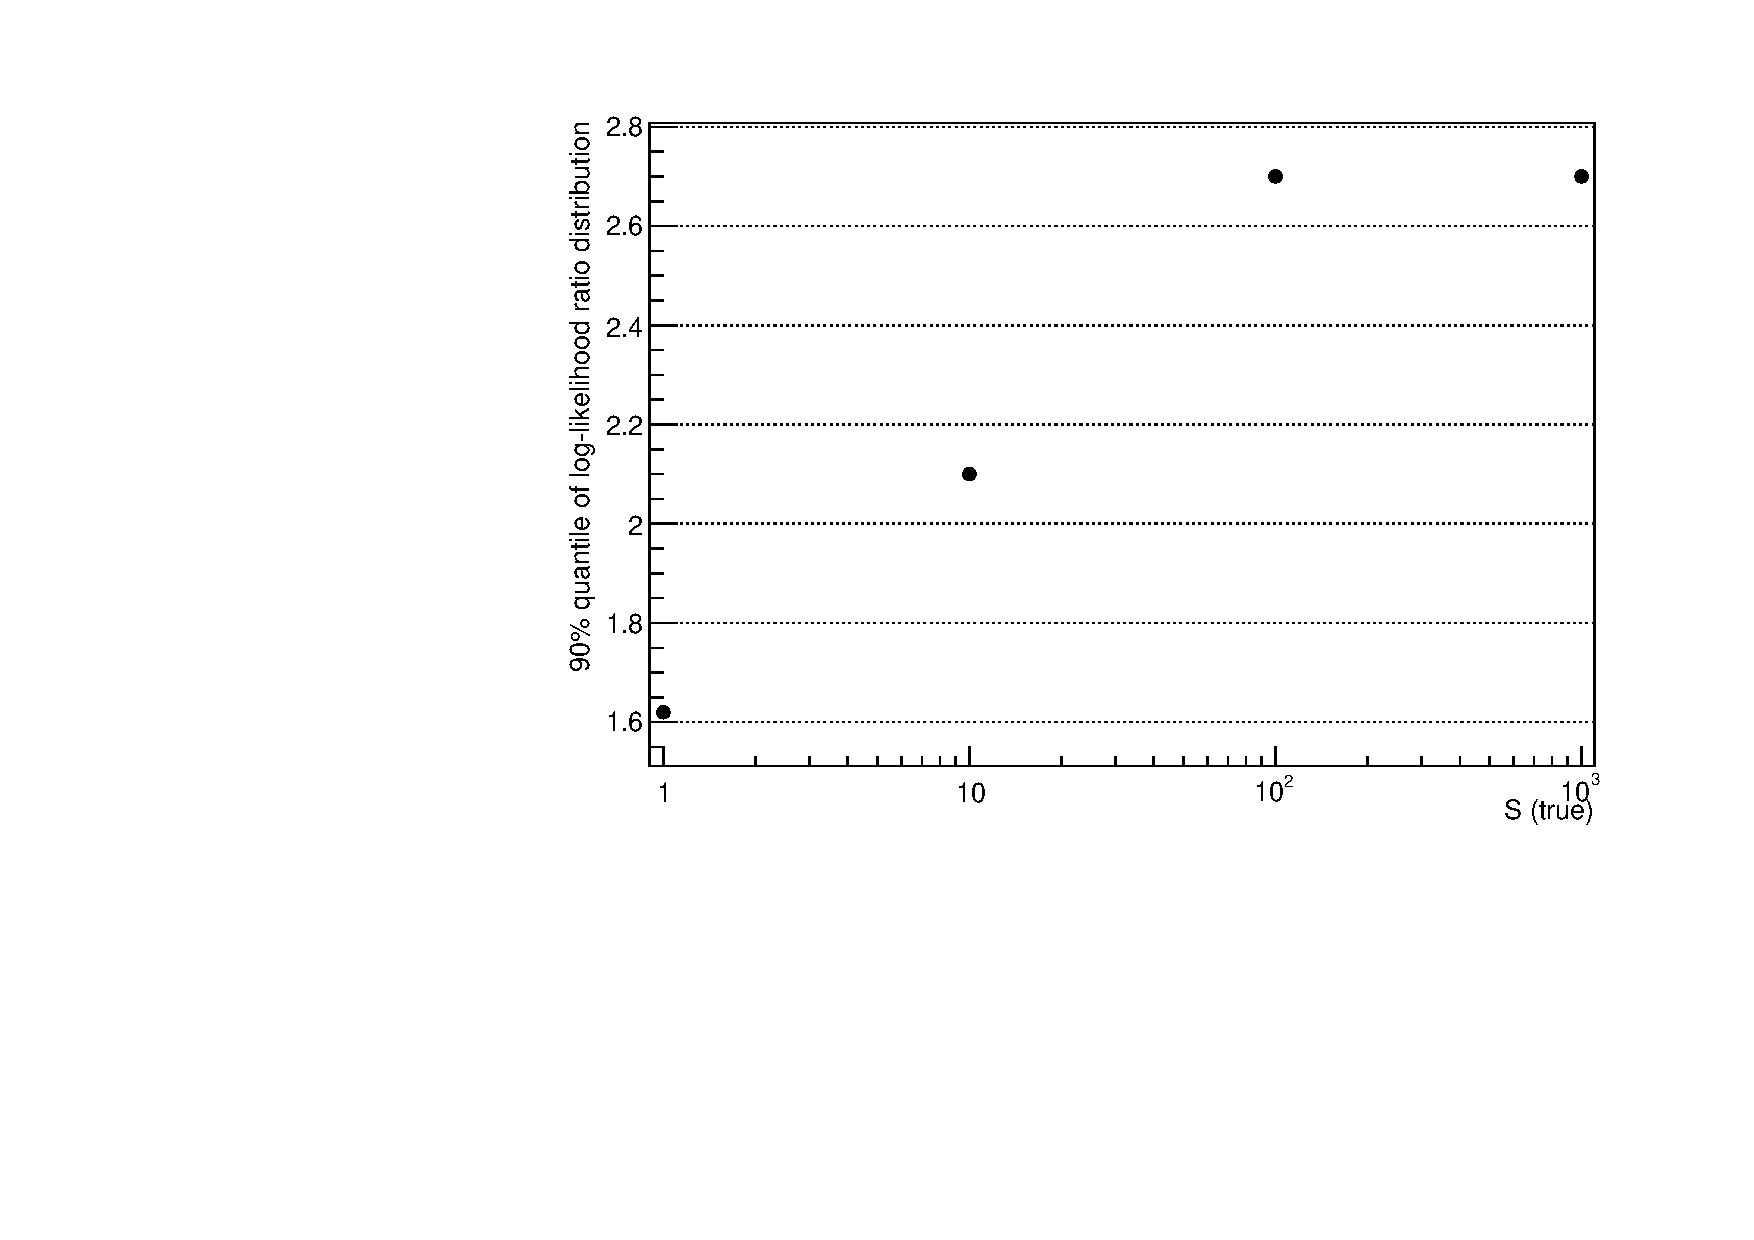
\includegraphics[width=\textwidth]{Ex2_threshold.pdf}
    \caption{$90\%$ quantile of the distribution of the log-likelihood ratio test statistics $t$ as a function of the injected signal $S (true)$ in a high background condition $B = 1000$. The $t$ distribution was obtained from a sample of $N_{toy} \geq 10^5$ toy-MC datasets.}
    \label{fig:threshold_b1000}
\end{figure}

\section{Sensitivity}
% make brazilian plot
Knowing (well) the amount of expected background, its shape and the signal shape, it is possible to compute the median sensitivity for limit-setting as a function of the expected (true) signal $S$ at a given confidence level $CL$. This statement can be made more clear: the log likelihood ratio test statistics is well defined given the shape of the signal and background and the signal $S$ for which we wish to compute the sensitivity. Then it is possible to compare the test statistics distribution in two different cases:
\begin{itemize}
\item null hypothesis $H_0$: signal $S$ and background $B$
\item alternate hypothesis $H_1$: background $B$ only
\end{itemize}
When performing the \textit{real} experiment one will not know a priori if the sample he extracted came from a universe with \textit{true} signal $S = S_{true}$ or from another one with $S=0$ (obviousely) and will perform an hypothesis test. Fixed a confidence level $CL$, he will reject the null hypothesis (i.e. exclude that particular signal expectation and put a more stringent limit) if the $p$-value of the data (computed assuming the null hypothesis, of course) is below the $1-CL$ threshold. The question the sensitivity analysis is willing to address is: "what  (median) $p$-value would the analyst compute if the background only hypothesis were true?". If this $p$-value is below the $1-CL$ level, the experiment will be (likely) able to put a limit on that signal strength. On the other hand, if the median $p$-value is above $1-CL$ then the experiment is not sensitive enough to that signal strength. That $p$-value is defined as the integral of the probability density function (pdf) of the log likelihood ratio test statistics ($t_S$) for the signal $S$ in the null (signal and background) hypothesis, from the median of the pdf $f(t_S | S_{true}=0)$ of that very same test statistics obtained in the alternate hypothesis, to infinity:

$$ p = \int_{t^*}^\infty f(t_S | S_{true} = S)dt_S \quad \mathrm{where} \quad \int_{-\infty}^{t^*} f(t_S | S_{true} = 0)dt_S = \int^{+\infty}_{t^*} f(t_S | S_{true} = 0)dt_S  $$

Sometimes in order to give an idea of how much the measured $p$-value is allowed to fluctuate around the median one, the so called brazilian plots are shown, where the green area corresponds to $1\sigma$ (i.e. $68.3\%$ probability content) and the yellow area to $2\sigma$ (i.e. $95\%$ probability content) of the $f(t_S|S_{true}=0)$ is shown. A very rough example is given in Fig. \ref{fig:brazil}. 
Due to the limited size of the sample ($N_{gen} = 10^6$ events) the median $p$-value for $S=100,1000$ is $0$ (and does not appear in the log scale).  This information is sufficient, though, to say that the experiment has a $90\% CL$ median sensitivity for limit setting for $S > 100$.
\begin{figure}[h]
    \centering
    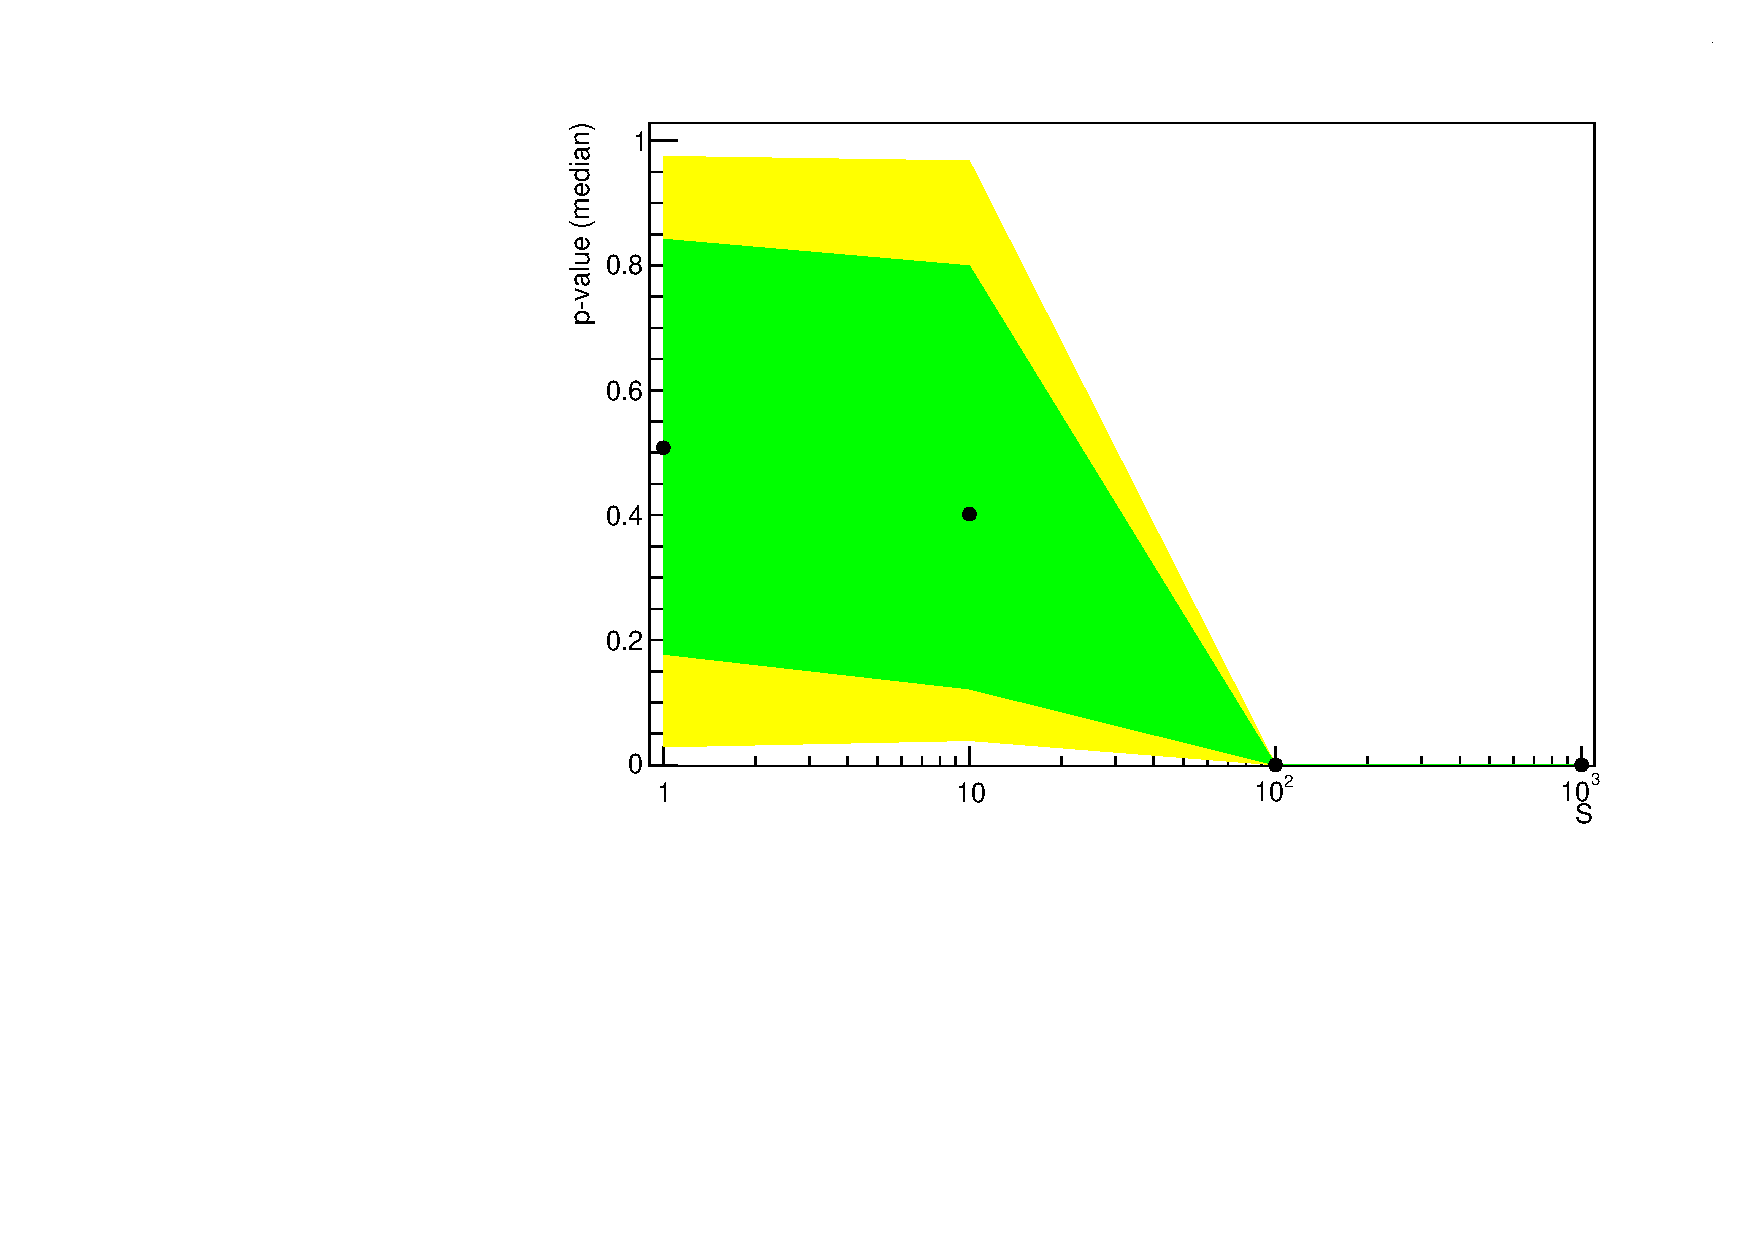
\includegraphics[width=0.49\textwidth]{brazil_lin.pdf} 
    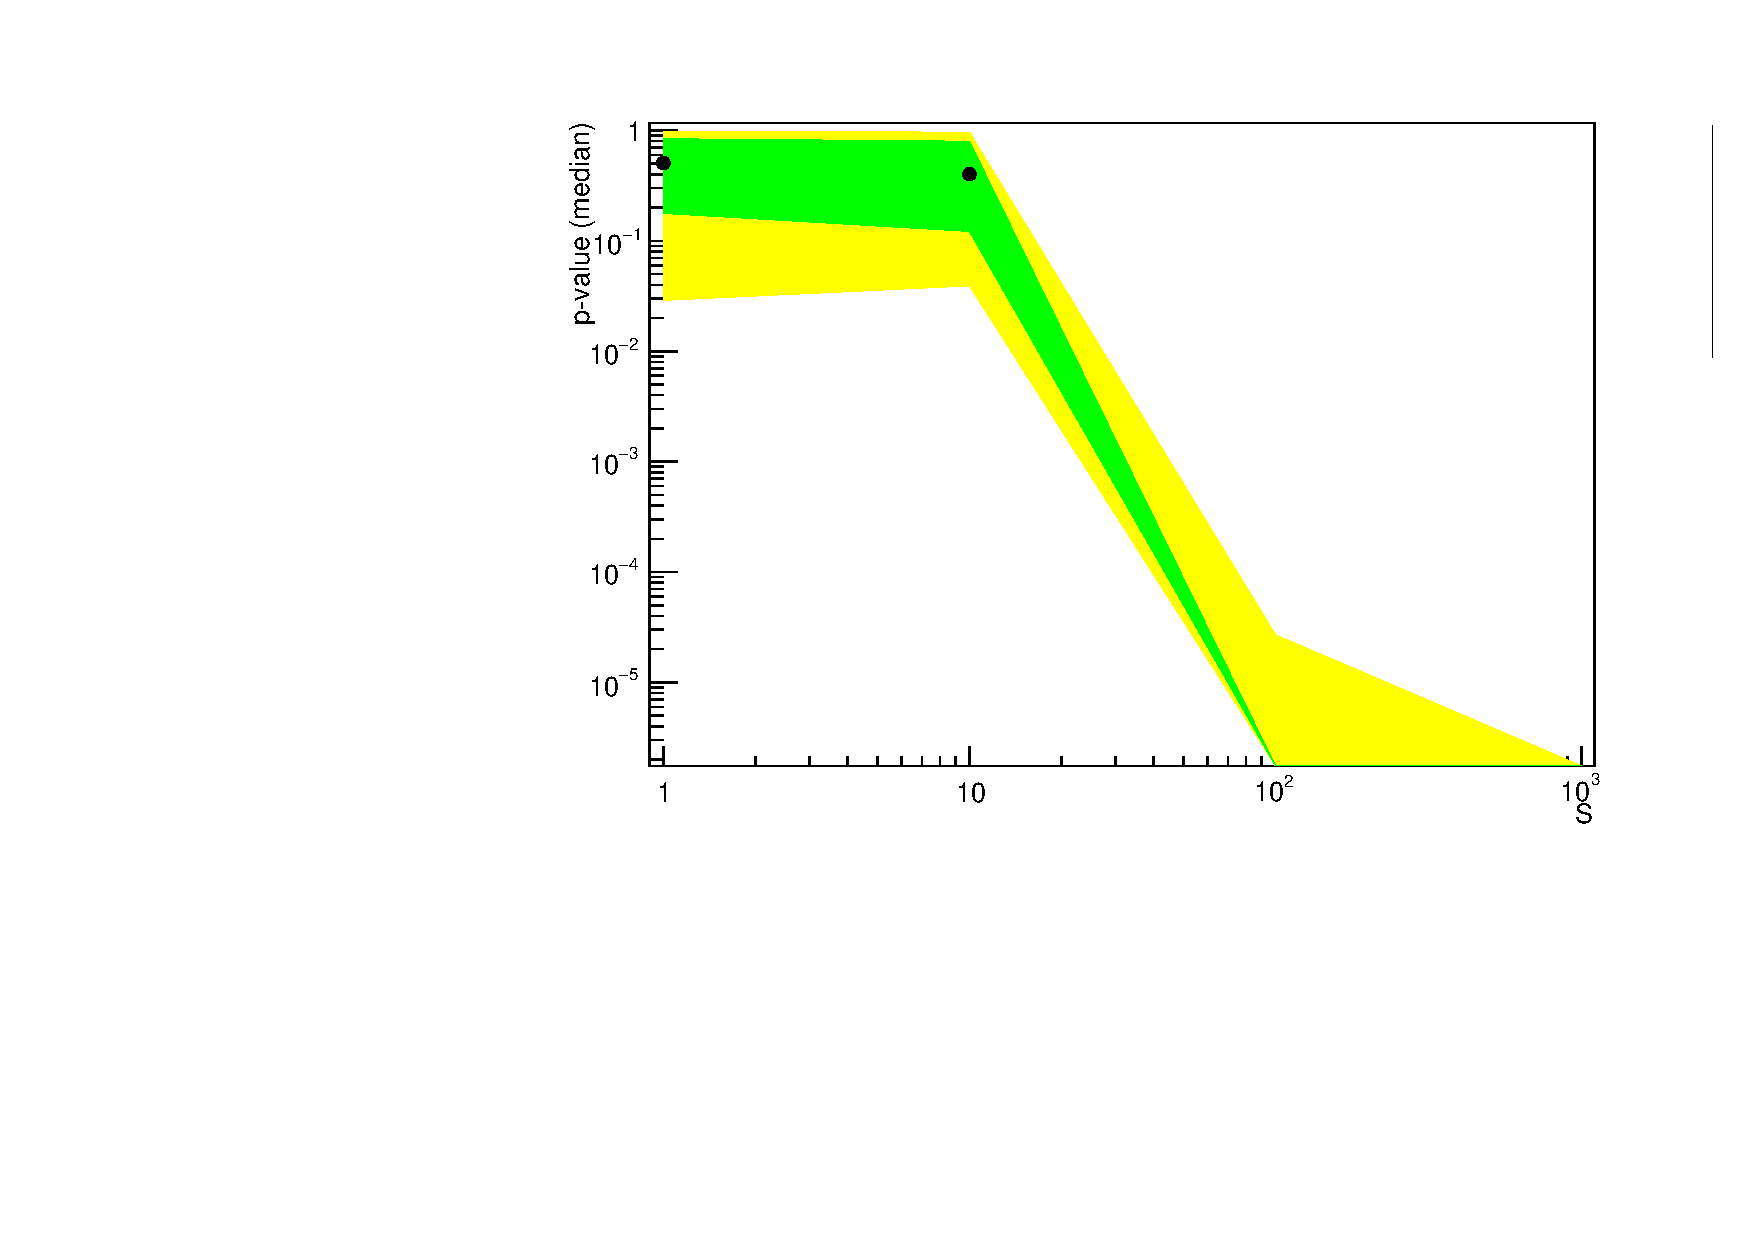
\includegraphics[width=0.49\textwidth]{brazil_log.pdf}
    \caption{Sensitivity curve (full circles indicate median $p$-value) for limit setting in high background conditions $B=1000$. The green (yellow) band show the $1\sigma (2\sigma)$ (probability content in the gaussian approximation) expected $p$-values.}
    \label{fig:brazil}
\end{figure}

\begin{figure}[h]
    \centering
    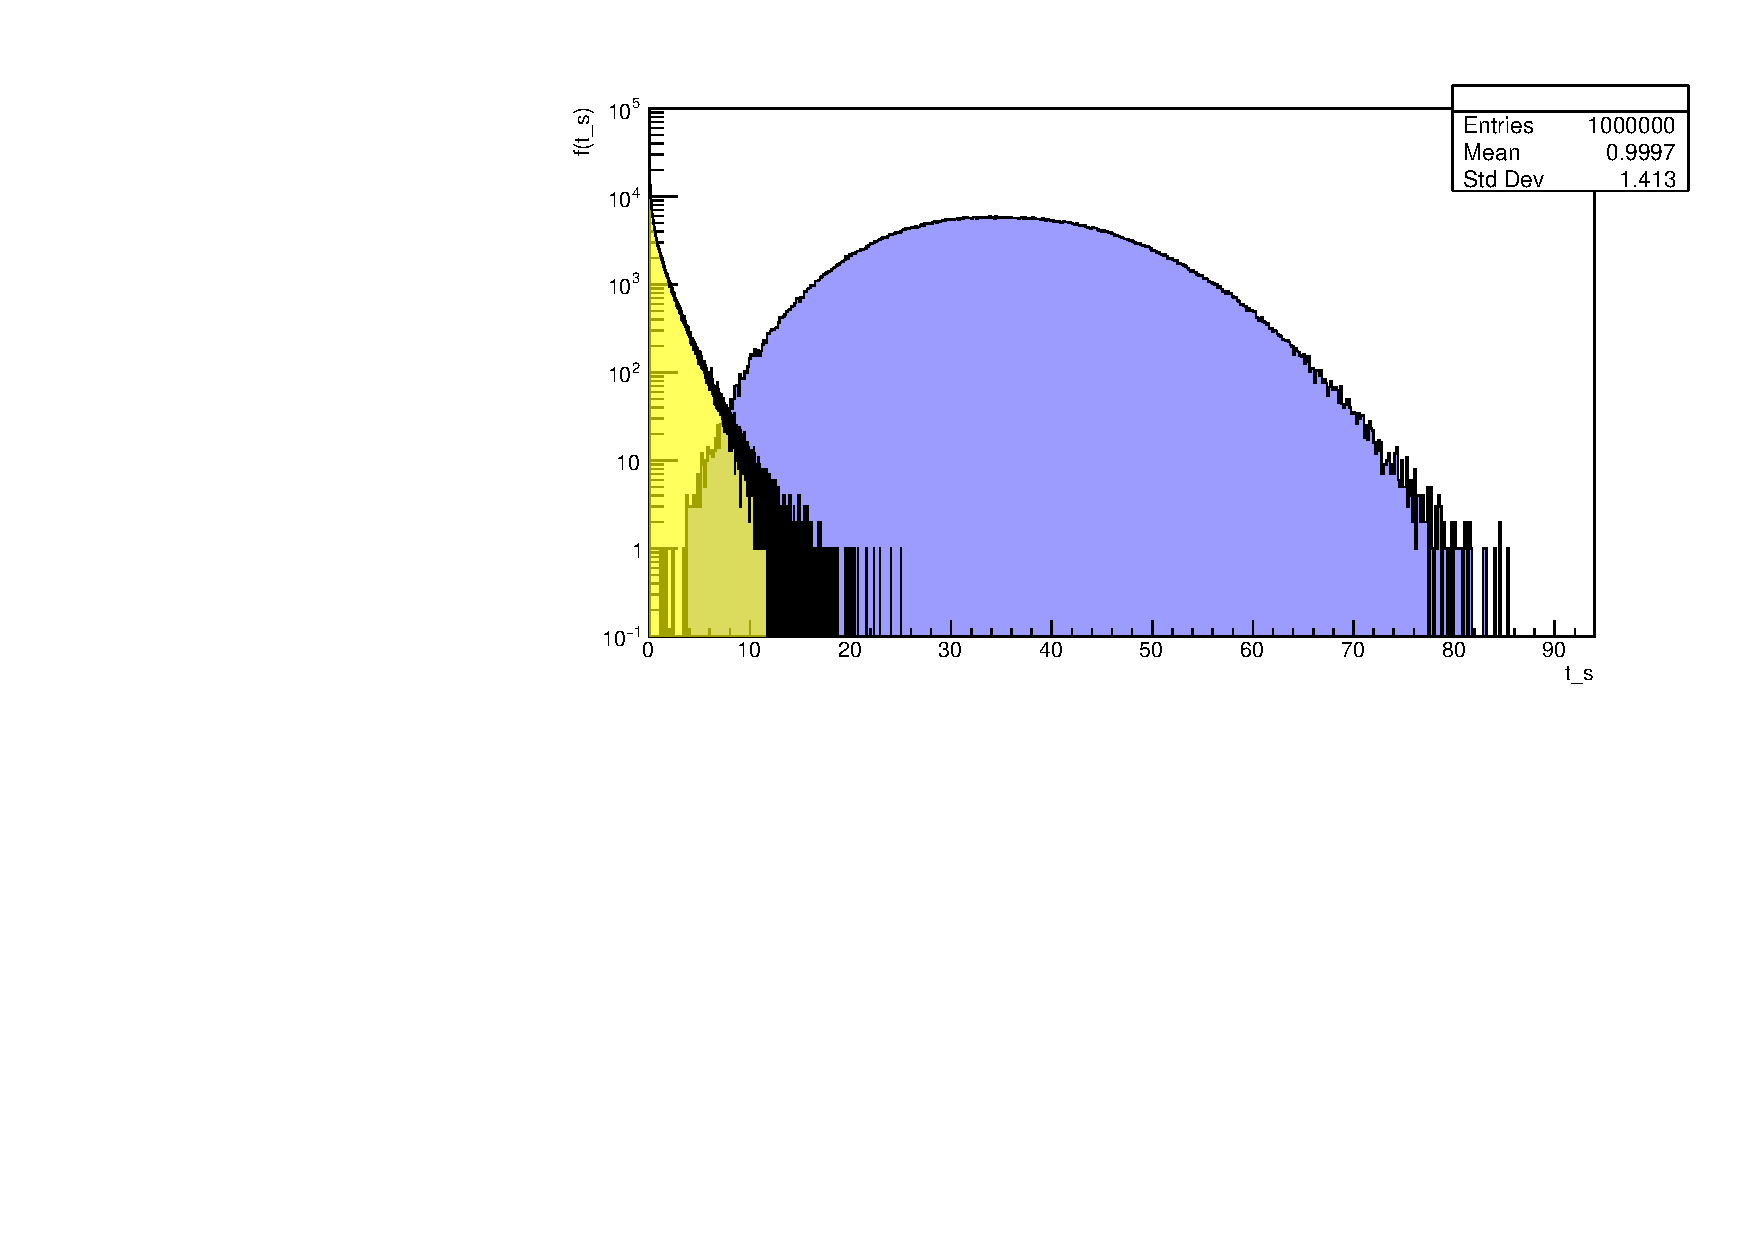
\includegraphics[width=\textwidth]{Ex3_B1000S100.pdf}
    \caption{Comparison of the log likelihood ratio test statistics $t_s$ for $S=100$ in the null hypothesis ($S_{true}=100$ and $B_{true}=1000$, yellow) and in the alternate hypothesis ($S_{true}=0$ and $B_{true} = 1000$, blue).}
    \label{fig:overlap_B1000S100N1e6}
\end{figure}

\section{Correlation and biases}
When a set of parameters is extracted from data it is important to check the correlations between them and to investigate possible biases of the fitting procedure. This was done generating $N_{toy} = 10^4$ datasets in three different conditions from a model defined by the sum of an exponentially decreasing background and two gaussian signals:

$$ f_{true} = (N1)_{true} \: \frac{1}{200} e^{-x/200} + (N2)_{true} \: g(m_{\mu}\cdot 50,m_{\sigma}\cdot 30) + (N3)_{true} \: g(m_{\mu}\cdot 60,m_{\sigma}\cdot 10)$$
where $x$ is a random variable (the observable), $g(\mu,\sigma)$ is a normalized gaussian distribution of mean $\mu$ and variance $\sigma^2$, and the $m$ coefficients are multipliers used to modify the mean and variance of the distribution in order to investigate the effect of this on the fit result. The generated datasets were always fit with the nominal model (i.e. $m_\mu = 1$ and $m_\sigma = 1$).
The three conditions taken into account are:
\begin{itemize}
\item $m_\mu = 1$ and $m_\sigma = 1$ (i.e. nominal conditions); the results are shown in Fig. \ref{fig:correlation_000}
\item $m_\mu = 1.01$ and $m_\sigma = 1$ (i.e. $+1\%$ shifted gaussian means, nominal $\sigma$); the results are shown in Fig. \ref{fig:correlation_001}	
\item $m_\mu = 1$ and $m_\sigma = 1.01$ (i.e. nominal gaussian means, $+1\%$ enlarged $\sigma$); the results are shown in Fig. \ref{fig:correlation_002}
\end{itemize}

\begin{figure}[h]
    \centering
    \includegraphics[width=\textwidth]{../out/Ex4/correlation_005.pdf}
    \caption{Outcome of the fit of $N_{toy} = 10^4$ generated datasets with $m_\mu = 1$ and $m_\sigma = 1$. In the diagonal plots a gaussian fit (red) is superimposed.}
    \label{fig:correlation_000}
\end{figure}
\begin{figure}[h]
    \centering
    \includegraphics[width=\textwidth]{../out/Ex4/correlation_006.pdf}
    \caption{Outcome of the fit of $N_{toy} = 10^4$ generated datasets with $m_\mu = 1.01$ and $m_\sigma = 1$. In the diagonal plots a gaussian fit (red) is superimposed.}
    \label{fig:correlation_001}
\end{figure}
\begin{figure}[h]
    \centering
    \includegraphics[width=\textwidth]{../out/Ex4/correlation_007.pdf}
    \caption{Outcome of the fit of $N_{toy} = 10^4$ generated datasets with $m_\mu = 1$ and $m_\sigma = 1.01$. In the diagonal plots a gaussian fit (red) is superimposed.}
    \label{fig:correlation_002}
\end{figure}



\paragraph{Comments}
The outcome of the fit, $(N1)_{fit}, (N2)_{fit}, (N3)_{fit}$ are random variables themselves, because they float randomly as the dataset changes. The aim of computing the toy Monte Carlo datasets is to properly sample from their distribution in order to understand the details of the fitting procedure. In particular:
\begin{itemize}
\item is the fit biased? In other words is $ b_i \doteq E[(Ni)_{fit}] - (Ni)_{true} \quad \mathrm{where} \quad i = 1,2,3$ different from zero?
\item are the parameters correlated?
\end{itemize}
The width of the distribution of the fit outcomes is an indication of the statistical uncertainty on the evaluated parameters.
In nominal conditions the bias for the number of signal counts is $b_2 = 0$ and $b_3 = 0$.
The statistical uncertainties are $\sigma_2 = 1.8 \cdot 10^3 \:\mathrm{counts} $ and $\sigma_3 = 8.8 \cdot 10^2 \:\mathrm{counts}$.
A mismatch between the model used to generate and the one used to fit the data introduces a bias. In fact a shift of $+1 \%$ of the mean value of the distributions used to fit the signal introduces a bias (see Fig. \ref{fig:correlation_001}) $b_2 = -1.6 \cdot 10^2$ and $b_3 = 0$.
A broadening of $+1\%$ of the standard deviation of both the gaussian distributions used in the fit (see Fig. \ref{fig:correlation_002}) introduces a bias $b_2 = +2 \cdot 10^2 \:\mathrm{counts}$ and $b_3 = 0$.

Since the statistical uncertainty on the $N2$ parameter is one order of magnitude bigger than the bias, in this case the bias can be neglected. In general one can express the uncertainty on a parameter $\theta$ with the \textit{main squared error} (MSE) defined as
$$ \mathrm{MSE}[\hat{\theta}] = b^2 + \mathrm{Var}^2[\hat{\theta}]$$
where $\hat{\theta}$ is the estimator of the $\theta$ parameter.

\end{document}

%---------------------------------------------------------------------------------